\documentclass[12pt,a4paper]{report}
\usepackage[english]{babel}
\usepackage{amssymb}
\usepackage{amsthm}
\usepackage{graphicx}
\usepackage{hyperref}
\usepackage[utf8]{inputenc}
\usepackage{mathtools}

\theoremstyle{plain}
\newtheorem{thm}{Theorem}[subsection] % reset theorem numbering for each chapter
\theoremstyle{definition}
\newtheorem{defn}[thm]{Definition} % definition numbers are dependent on theorem numbers
\newtheorem{exmp}[thm]{Example} % same for example numbers
\newtheorem{prf}[thm]{Proof} % same for proof numbers
\newtheorem{rem}[thm]{Remark} % same for remark numbers

\begin{document}
	\begin{titlepage} % Suppresses headers and footers on the title page
		
		\centering % Centre everything on the title page
		
		\scshape % Use small caps for all text on the title page
		
		%------------------------------------------------
		%	Title
		%------------------------------------------------
		
		\rule{\textwidth}{1.6pt}\vspace*{-\baselineskip}\vspace*{2pt} % Thick horizontal rule
		\rule{\textwidth}{0.4pt} % Thin horizontal rule
		
		\vspace{0.75\baselineskip} % Whitespace above the title
		
		{Comparison of multi-signature schemes for performance improvement of OmniLedger} % Title
		
		\vspace{0.75\baselineskip} % Whitespace below the title
		
		\rule{\textwidth}{0.4pt}\vspace*{-\baselineskip}\vspace{3.2pt} % Thin horizontal rule
		\rule{\textwidth}{1.6pt} % Thick horizontal rule
		
		\vspace{2\baselineskip} % Whitespace after the title block
		
		%------------------------------------------------
		%	Subtitle
		%------------------------------------------------
		
		Bachelor thesis for the department of Mathematics of Utrecht University % Subtitle or further description
		
		\vspace*{3\baselineskip} % Whitespace under the subtitle
		
		%------------------------------------------------
		%	Author
		%------------------------------------------------
		
		Student
		
		\vspace{0.5\baselineskip} % Whitespace before the editors		
		{\scshape\Large Paul van Grol} % Editor list
		
		\vspace{0.5\baselineskip} % Whitespace below the editor list
		
		\textit{Utrecht University} % Editor affiliation
		
		\vspace*{2\baselineskip} % Whitespace under the subtitle
		
		%------------------------------------------------
		%	Author
		%------------------------------------------------
		
		Primary supervisor
		
		\vspace{0.5\baselineskip} % Whitespace before the editors
		
		{\scshape\Large Veelasha Moonsamy} % Editor list
		
		\vspace{0.5\baselineskip} % Whitespace below the editor list
		
		\textit{Utrecht University} % Editor affiliation
		
		\vspace*{1\baselineskip} % Whitespace under the subtitle
		
		%------------------------------------------------
		%	Author
		%------------------------------------------------
		
		Secondary supervisor
		
		\vspace{0.5\baselineskip} % Whitespace before the editors
		
		{\scshape\Large Damaris Schindler} % Editor list
		
		\vspace{0.5\baselineskip} % Whitespace below the editor list
		
		\textit{Utrecht University} % Editor affiliation
		
		\vspace{3\baselineskip} % Whitespace below the editor list
		
		\today
		
		
\includegraphics{UU_logo_EN_CMYK}
	\end{titlepage}
	\begin{abstract}
		There is an ever increasing amount of users of distributed ledger systems, such as blockchains. The systems do, however, not scale in performance with an increase in participants.
		
		OmniLedger addresses that problem by introducing sharding to distributed ledger systems, to allow for asynchronous handling of transactions to increase system performance.
		
		This thesis studies two multi-signature schemes in order to further improve the performance of OmniLedger. The BLS multi-signature scheme that is based on the Weil pairing on elliptic curves, and MuSig, a Schnorr-based multi-signature scheme.
		
		The conclusion of this thesis is that BLS is the superior choice to improve OmniLedger, for it offers greater performance and stability.
	\end{abstract}
	\tableofcontents
	\documentclass[12pt]{report}
\usepackage[backend=bibtex8]{biblatex}
\usepackage[utf8]{inputenc}

\addbibresource{references.bib}
\begin{document}
	\chapter{Introduction}
	This thesis has been inspired by a recent paper that introduced OmniLedger\cite{omniledger}: a scalable, decentralized ledger. In a world where more and more uses are found for blockchain technology, the promise of such a technology that scales in performance with the amount of users is incredibly interesting. Considering that current systems might actually perform worse when the amount of users increases, it is interesting to look at OmniLedger to see whether it can help in that regard.
	
	In particular, this thesis focusses on multi-signature algorithms that may be used to improve the performance of RandHound\cite{randhound}. RandHound is used by OmniLedger to ensure that the system remains uncompromised. Since evaluation has shown that RandHound takes up more than 70\% of the total runtime in the bootstrap process of OmniLedger, which happens periodically, improving the performance of RandHound should lead to an improvement in performance of OmniLedger.
	\\
	\\
	Therefore the research question of this thesis is as follows: " .. ". To answer this question, some background is needed, before comparisons can be made between various multi-signature algorithms.
	
	As such the second chapter introduces algebraic varieties, leading up to an explanation of elliptic curves and some properties that are used to great effect in cryptography. The chapter concludes with an explanation of the Weil pairing on elliptic curves, which is used in one of the multi-signature algorithms used.
	
	The third chapter then introduces the technological background of ledgers, blockchain and multi-signatures among other terms and concepts used to clearly show the context of the research.
	
	In chapter four and five two different multi-signature algorithms are studied, leading up to the comparison of them in chapter six and the conclusion as to the most suitable choice for RandHound.
\end{document}

	\chapter{Mathematical Background}
This chapter provides the mathematical background to elliptic curve cryptography. If the reader is already familiar with elliptic curves and the Weil pairing, skipping to the section on elliptic curve cryptography should not hinder the understanding of that chapter. If the reader is unfamiliar, or wishes to refresh his memory, reading this chapter is advised.

A background in and understanding of fields, rings and Galois groups is assumed in this chapter.

This chapter will start with algebraic varieties and lead up to elliptic curves and the Weil pairing, finishing with an explanation of elliptic curve cryptography.

As source material in this chapter, the excellent work of Joseph H. Silverman is used \cite[Chapter 1-3]{EllipticCurvesBook}, along with some of his slides \cite{EllipticCurvesSlides}.

\section{Algebraic Varieties}
\subsection{Notation}
Before explaining algebraic varieties, the following notation is set.
\begin{itemize}
	\item $K$ is a perfect field.
	\item $\bar{K}$ is a fixed algebraic closure of $K$.
	\item $\bar{K}[X]=\bar{K}[X_1,\dots,X_n]$ is a polynomial ring in $n$ variables.
	\item $G_{\bar{K}/K}$ is the Galois group of $\bar{K}/K$.
\end{itemize}

\subsection{Affine Varieties}
The following definition defines Cartesian $n$-space and the subsets that are defined by zeros of polynomials.
\begin{defn}
	Cartesian, also known as affine, $n$-space, which is implied to be over $K$, is the set of $n$-tuples.
	\begin{equation*}
	\mathbb{A}^n=\mathbb{A}^n(\bar{K})=\{P=(x_1,\dots,x_n):x_i\in\bar{K}\}
	\end{equation*}
	This leads to the set of $K$-rational points of $\mathbb{A}^n$ as the following set.
	
	\begin{equation*}\mathbb{A}^n(K)=\{P=(x_1,\dots,x_n)\in\mathbb{A}^n:x_i\in K\}
	\end{equation*}
\end{defn}

From this point on, any space used is, indeed, an affine space. Using the Galois group $G_{\bar{K}/K}$ allows for an alternative description of $\mathbb{A}^n(K)$, because the Galois group fixes elements $P\in\mathbb{A}^n$.
\begin{rem}
	Considering the Galois group $G_{\bar{K}/K}$ leads to an action on $\mathbb{A}^n$ such that for $\sigma\in G_{\bar{K}/K}$ and $P\in\mathbb{A}^n$, it leads to
	\begin{equation*}
	P^\sigma=(x_1^\sigma,\dots,x_n^\sigma).
	\end{equation*}
	This then allows to define $\mathbb{A}^n(K)$ as
	\begin{equation*}
	\mathbb{A}^n(K)=\{P\in\mathbb{A}^n:P^\sigma=P,\forall\sigma\in G_{\bar{K}/K}\}.
	\end{equation*}
\end{rem}

Using ideals in $\bar{K}[X]$ leads to the construction of an algebraic set on $\mathbb{A}^n$.
\begin{defn}
	Taking $I\subset\bar{K}[X]$ as an ideal, each of these can be associated with a subset of $\mathbb{A}^n$ such that
	\begin{equation*}
	V_I=\{P\in\mathbb{A}^n:f(P)=0,\forall f\in I\}.
	\end{equation*}
	Any set of this form is an algebraic set.
\end{defn}

On an algebraic set, in turn, the ideal may be defined.
\begin{defn}
	Given an algebraic set V, the ideal of V is
	\begin{equation*}
	I(V)=\{f\in\bar{K}[X]:f(P)=0,\forall P\in V\}.
	\end{equation*}	
\end{defn}
If $I(V)$ can be generated by polynomials in $K[X]$ for an algebraic set $V$, it is defined over $K$ and noted as $V/K$.

Using an algebraic set $V$ and the corresponding ideal $I(V)$ leads to the definition of an affine variety.
\begin{defn}
	$V$ is called an affine variety if $I(V)$ is a prime ideal in $\bar{K}[X]$.
\end{defn}

\subsection{Projective Varieties}
Making an affine space a projective space is done by adding the so called ``points at infinity". This same process can be recreated to define projective varieties.
\begin{defn}
	$\mathbb{P}^n=\mathbb{P}^n(\bar{K})$ denotes the projective $n$-space over $K$ and is constructed as the set of all $(n+1)$ tuples
	\begin{equation*}
	(x_0,\dots,x_n)\in\mathbb{A}^{n+1}.
	\end{equation*}
	
	These tuples must be such that at least one element is nonzero modulo the following equivalence relation
	\begin{equation*}
	(x_0,\dots,x_n)\sim(y_0,\dots,y_n)
	\end{equation*}
	
	if there is a $\lambda\in\bar{K}^*$ such that $x_i=\lambda y_i,\forall i$. The resulting equivalence class
	\begin{equation*}
	\{(\lambda x_0,\dots,\lambda x_n):\lambda\in\bar{K}^*\}
	\end{equation*}
	
	is noted as $[x_0,\dots,x_n]$, with the elements being called homogeneous coordinates for the point $P\in\mathbb{P}^n$ that corresponds to it. This leads to the set of $K$-rational points in $\mathbb{P}^n$
	\begin{equation*}
	\mathbb{P}^n(K)=\{[x_0,\dots,x_n]\in\mathbb{P}^n:x_i\in K\}
	\end{equation*}
\end{defn}
As with affine varieties, the Galois group $G_{\bar{K}/K}$ allows for an alternate definition of $\mathbb{P}^n(K)$.
\begin{rem}
	The Galois group $G_{\bar{K}/K}$ acts on $P\in\mathbb{P}^n$ via
	\begin{equation*}
	[x_0,\dots,x_n]^\sigma=[x_0^\sigma,\dots,x_n^\sigma]
	\end{equation*}
	and as such it leads to
	\begin{equation*}
	\mathbb{P}^n(K)=\{P\in\mathbb{P}^n:P^\sigma=P,\forall\sigma\in G_{\bar{K}/K}\}
	\end{equation*}
\end{rem}

With the existence homogeneous coordinates, homogeneous polynomials and ideals can be defined.
\begin{defn}
	A polynomial $f\in\bar{K}[X]$ is homogeneous of degree $d$ if
	\begin{equation*}
	f(\lambda X_0,\dots,\lambda X_n)=\lambda^df(X_0,\dots,X_n),\forall \lambda\in\bar{K}
	\end{equation*}
	An ideal $I\subset\bar{K}[X]$ is homogeneous if it is generated by homogeneous polynomials.
\end{defn}

With $f$ a homogeneous polynomial, it is interesting to look at points $P\in\mathbb{P}^n$ where $f(P)=0$. Using these points, for each homogeneous ideal $I$ a subset can be defined.
\begin{defn}
	Taking $f$ to be a homogeneous polynomial, any set of the following form for a homogeneous ideal $I$ is a projective algebraic set.
	\begin{equation*}
	V_I=\{P\in\mathbb{P}^n:f(P)=0,\forall f\in I\}
	\end{equation*}
\end{defn}

Such a set has, of itself, a homogeneous ideal.
\begin{defn}
	$I(V)$, the homogeneous ideal of $V$ is the ideal of $\bar{K}[X]$ that is generated with homogeneous $f$ by
	\begin{equation*}
	\{f\in\bar{K}[X]:f(P)=0,\forall P\in V\}
	\end{equation*}
\end{defn}

The homogeneous ideal is used to define a projective variety.
\begin{defn}
	If the homogeneous ideal $I(V)$ of projective algebraic set $V_I$ is a prime ideal in $\bar{K}[X]$, the set $V_I$ is called a projective variety.
\end{defn}
\section{Elliptic Curves}
An elliptic curve is an algebraic curve of genus one with a certain base point. This section will begin with elliptic curves given by Weierstrass equations, explain the group action on elliptic curves, then look at arbitrary elliptic curves and show that all have a Weierstrass equation study the Weil pairing on elliptic curves. The final section will explain elliptic curve cryptography and give some uses.
\subsection{Weierstrass Equations}
The Weierstrass equation for elliptic curves is written as as follows
\begin{defn}
	Given a base point $O$ and $a_1,\dots,a_6\in\bar{K}$ the Weierstrass equation for an elliptic curve is
	\begin{equation*}
	Y^2Z+a_1XYZ+a_3YZ^2=X^3+a_2X^2Z+a_4XZ^2+a_6Z^3.
	\end{equation*}
	This is generally written with non-homogeneous coordinates $x=X/Z$ and $y=Y$
	\begin{equation*}
	E:y^2+a_1xy+a_3y=x^3+a_2x^2+a_4x+a_6.
	\end{equation*}
	If $a_1,\dots,a_6\in K$, $E$ is said to be defined over $K$.
\end{defn}

If $char(\bar{K})\neq 2$, then this equation an be simplified further by substituting
\begin{equation*}
y=\frac{1}{2}(y-a_1x-a_3).
\end{equation*}

This leads to the following equation
\begin{equation*}
E:y^2=4x^3+b_2x^2+2b_4x+b_6
\end{equation*}

where
\begin{equation*}
{b_2=a_1^2+4a_2}\text{,		}{b_4=2a_4+a_1a_3}\text{,	}{b_6=a_3^2+4a_6}.
\end{equation*}

Furthermore define
\begin{equation*}
b_8=a_1^2a_6+4a_2a_6-a_1a_3a_4+a_2a_3^2-a_4^2,
\end{equation*}
\begin{equation*}
c_4=b_2^2-24b_4,
\end{equation*}
\begin{equation*}
c_6=-b_2^3+36b_2b_4-216b_6,
\end{equation*}
\begin{equation*}
\Delta=-b_2^2-8b_4^3-27b_6^2+9b_2b_4b_6,
\end{equation*}
\begin{equation*}
j=c_4^3/\Delta,
\end{equation*}
\begin{equation*}
\omega=\frac{dx}{2y+a_1x+a_3}=\frac{dy}{3x^2+2a_2x+a_4-a_1y}.
\end{equation*}


Using those, it is easy to see that
\begin{equation*}
4b_8=b_2b_6-b_4^2\text{ and }1728\Delta=c_4^3-c_6^2.
\end{equation*}


If $char(\bar{K})\neq 2,3$, the substitution
\begin{equation*}
(x,y)=(\frac{x-3b_2}{36},\frac{y}{108})
\end{equation*}

allows to eliminate $x^2$, leaving the simple equation
\begin{equation*}
E:y^2=x^3-27c_4x-54c_6.
\end{equation*}

Some of the previously defined quantities have specific meanings.
\begin{defn}
	The value $\Delta$ is the discriminant of the Weierstrass equation, $j$ is the $j$-invariant of the elliptic curve and $\omega$ is the invariant differential that is associated with the Weierstrass equation.
\end{defn}

Because $27c_4$ and $54c_6$ are simple values, the Weierstrass equation of an elliptic curve when the characteristic of $K$ is not 2 or 3 is
\begin{equation*}
E:y^2=x^3+Ax+B.
\end{equation*}

In this case it follows that
\begin{equation*}
\Delta=-16(4A^3+27B^2)\text{ and }j=-1728\frac{(4A)^3}{\Delta}.
\end{equation*}

\subsection{Group Action}
In this section the elliptic curve $E$ is given by a Weierstrass equation. As such, $E\subset\mathbb{P}^2$ consists of points $P=(x,y)$ satisfying
\begin{equation*}
f(x,y)=y^2+a_1xy+a_3y-x^3-a_2x^2-a_4x-a_6=0
\end{equation*}

It is easy to see that the equation has degree three, and that, as such, there are three points of interesection for line $L\subset\mathbb{P}^2$. These points $P,Q,R$ need not be distinct, since $L$ may be a tangent. Using this, the composition law $\oplus$ on $E$ is defined as follows.
\begin{defn}
	Let $P,Q\in E$ and let $L$ be the line through $P$ and $Q$ if the points are distinct, or the tangent to $E$ at $P$ if $P=Q$. Let $R$ be the other point of intersection of $L$ with $E$. Denote by $L'$ the line through $R$ and $O$. Now $L'$ intersects $E$ at $R,O$ and a third point denoted by $P\oplus Q$.
\end{defn}
Now the usage of the symbol is justified by showing that it makes $E$ into an abelian group with identity $O$.
\begin{thm}
	The composition law $\oplus$ has the following properties:
	\begin{enumerate}
		\item If line $L$ intersects $E$ at points $P,Q,R$, not necessarily distinct, then
		\begin{equation*}
		(P\oplus Q)\oplus R=O
		\end{equation*}
		\item $P\oplus O=P\text{\space}\forall P\in E$
		\item $P\oplus Q=Q\oplus P\text{\space}\forall P,Q\in E$
		\item Given $P\in E$ there is a point of $E$, denoted $\ominus P$, such that
		\begin{equation*}
		P\oplus(\ominus P)=O
		\end{equation*}
		\item Given $P,Q,R\in E$
		\begin{equation*}
		(P\oplus Q)\oplus R=P\oplus(Q\oplus R)
		\end{equation*}
		\item Suppose that $E$ is defined over $K$, then the following is a subgroup of $E$
		\begin{equation*}
		E(K)=\{(x,y)\in K^2:y^2+a_1xy+a_3x^2+a_4x+a_6\}\cup\{O\}.
		\end{equation*}
	\end{enumerate}
\end{thm}
\begin{prf}
	\begin{enumerate}
		\item From the definition it follows that the line $L'$ used to construct $P\oplus Q$ intersects $E$ at $R,O$ and $P\oplus Q$. Therefore the intersection point is $O$, and the line through $O$ and $O$ ends up in $O$. In other words, the tangent line to $E$ at $O$ intersects $E$ at $O$ with multiplicity 3.
		\item Note that in this case, the lines $L$ and $L'$ are the same, and that as such the intersection of the line through $O$ and $P\oplus O$ intersects $E$ at precisely $P$.
		\item It is easy to see that the construction of $P\oplus Q$ is symmetric in both $P$ and $Q$. The line through two points that remain fixed does not depend on the order in which the points are picked.
		\item Take a line through $P$ and $O$ and call the intersection point $R$. Using $1.$ and $2.$ it is easy to see that $O=(P\oplus O)\oplus R=P\oplus R.$
		\item This proof will be handled later with explicit formulas.
		\item If both $P$ and $Q$ have coordinates in $K$, then the coefficients of the equation of the line $L$ connecting $P$ and $Q$ are in $K$. If, furthermore, $E$ is defined over $K$ then the third point will be a ratinal combination of coefficients of the line and of $E$, and will thus be in $K$.
	\end{enumerate}
\end{prf}
\begin{rem}
	Since it has been proven that $\oplus$ is a group operation, this thesis will from now on use $+$ instead, and $-$ for $\ominus$. Furthermore, define $mP=\overbrace{P+\dots+P}^m$ if $m>0$, $mP=\overbrace{-P-\dots-P}^m$ if $m<0$ and $0P=O$.
\end{rem}

\subsection{Explicit Formulas}
The various group operations can also be expressed in explicit formulas, which will be derived in this section.
\begin{thm}
	Let $E$ be an elliptic curve given by the Weierstrass equation
	\begin{equation*}
	f(x,y)=y^2+a_1xy+a_3y-x^3-a_2x^2-a_4x-a_6=0,
	\end{equation*}
	\begin{enumerate}
		\item Let $P_0=(x_0,y_0)\in E$. Then
		\begin{equation*}
		-P_0=(x_0,-y_0-a_1x_0-a_3).
		\end{equation*}
		Now let $P_1+P_2=P_3$ with $P_i=(x_i,y_i)\in E$.
		\item If $x_1=x_2$ and $y_1+y_2+a_1x_2+a_3=0$ then
		\begin{equation*}
		P_1+P_2=0.
		\end{equation*}
		If this is not the case, define for $x_1\neq x_2$
		\begin{equation*}
		\lambda=\frac{y_2-y_1}{x_2-x_1}\text{ and }\nu=\frac{y_1x_2-y_2x_1}{x_2-x_1}
		\end{equation*}
		and for $x_1=x_2$
		\begin{equation*}
		\lambda=\frac{3x_1^2+2a_2x_1+a_4-a_1y_1}{2y_1+a_1x_1+a_3}\text{ and }\nu=\frac{-x_1^3+a_4x_1+2a_6-a_3y_1}{2y_1+a_1x_1+a_3}
		\end{equation*}
		Then $y=\lambda x+\nu$ is the line through $P_1$ and $P_2$.
		\item Using the same notation as $2.$, the coordinates for $P_3=P_1+P_2$ are
		\begin{equation*}
		(x_3=\lambda^2+a_1\lambda-a_2-x_1-x_2,y_3=-(\lambda+a_1)x_3-\nu-a_3)
		\end{equation*}
	\end{enumerate}
\end{thm}

\begin{prf}
	tba
\end{prf}

\subsection{Elliptic Curves}
This part will focus on linking Weierstrass equations to generic elliptic curves, to show that the results achieved for Weierstrass equations apply generally.
\begin{defn}
	An elliptic curve is a pair $(E,O)$, with $E$ a nonsingular curve of genus one, and $O\in E$. The elliptic curve $E$ is defined over $K$, written as $E/K$, if $E$ is defined over $K$ and $O\in E(K)$.
\end{defn}

To show that elliptic curves and Weierstrass equations are linked the Riemann-Roch theorem is used. See \cite{RiemannRoch} for a proof.
\begin{thm}[Riemann-Roch]
	Let $C$ be a smooth curve and let $K_C$ be a canonical divisor on $C$. There is an integer $g\geq0$, called the genus of $C$, such that for every divisor $D\in Div(C)$,
	\begin{equation*}
	\ell(D)-\ell(K_C-D)=deg(D)-g+1
	\end{equation*}
\end{thm}

\begin{thm}
	Let $E$ be an elliptic curve defined over $K$, then there exist functions $x,y\in K(E)$ such that the map
	\begin{equation*}
		\phi:e\to\mathbb{P}^2\text{ , }\phi=[x,y,1]
	\end{equation*}
	gives an isomorphism of $E/K$ onto a curve given by the Weierstrass equation
	\begin{equation*}
	C:Y^2+a_1XY+a_3Y=X^3+a_2X^2+a_4X+a_6
	\end{equation*}
	satisfying $\phi(O)=[0,1,0]$. The functions $x$ and $y$ are called the Weierstrass coordinates for the elliptic curve $E$
\end{thm}

This proof will show that the image of the map is indeed in $C$ as described by the Weierstrass equation. The rest of the proof may be found in \cite[page 60]{EllipticCurvesBook}
\begin{prf}
	tba
\end{prf}

\subsection{Weil Pairing}
The Weil pairing will be the last of the mathematical background discussed. This pairing uses $E_m$, the group of $m$-torsion points and $\mu_m$, the group of $m$-th roots of unity.
\begin{defn}
	Setting, for $X\in E$ and $g\in\bar{K}(E)$
	\begin{equation*}
	E_m(S,T)=\frac{g(X+S)}{g(X)}
	\end{equation*}
	the Weil pairing is a non-degenerate alternating bilineair form
	\begin{equation*}
	e_m=E_m\times E_m\to\mu_m
	\end{equation*}
\end{defn}
This pairing has the following properties
\begin{thm}
	The Weil $e_m$ pairing has these properties
	\begin{enumerate}
		\item The pairing is bilinear
		\begin{equation*}
		e_m(S_1+S_2,T)=e_m(S_1,T)e_m(S_2,T),
		\end{equation*}
		\begin{equation*}
		e_m(S,T_1+T_2)=e_m(S,T_1)e_m(S,T_2),
		\end{equation*}
		\item The pairing is alternating
		\begin{equation*}
		e_m(T,T)=1
		\end{equation*}
		which means in particular that
		\begin{equation*}
		e_m(S,T)=e_m(T,S)^{-1}
		\end{equation*}
		\item The pairing is nondegenerate
		\begin{equation*}
		\text{If } e_m(S,T)=1\text{ for all } S\in E_m\text{, then } T=O
		\end{equation*}
		\item The pairing is Galois invariant
		\begin{equation*}
		e_m(S,T)^\sigma=e_m(S^\sigma,T^\sigma)\text{ for all }\sigma\in G_{\bar{K}/K}
		\end{equation*}
		\item The pairing is compatible
		\begin{equation*}
		e_{mm'}(S,T)=e_m(m'S,T)\text{ for all }S\in E_{mm'}\text{ and }T\in E_m
		\end{equation*}
	\end{enumerate}
\end{thm}

\begin{prf}
	\begin{enumerate}
		\item tba
		\item tba
		\item tba
	\end{enumerate}
\end{prf}
The resulting proofs may be found in \cite[page 96]{EllipticCurvesBook} but are not of particular interest in this thesis.

\section{Discrete Logarithm Problem}
On the set of real numbers ($\mathbb{R}$) the $\log_b$ function has been defined as the solution to the following problem.
\begin{defn}
	Given $a,b,n\in\mathbb{R}$, base $b$ and power $a$ of $b$, what is n such that $a=b^n$?
\end{defn}
This same problem can also be defined over modulo $p$, which is known as the discrete logarithm problem over $\mathbb{Z}/p\mathbb{Z}$.
\begin{defn}[Discrete Logarithm Problem over $\mathbb{Z}/p\mathbb{Z}$]
	Given $a,b\in\mathbb{Z}/p\mathbb{Z}$, base $b$ and power $a$ of $b$, what is n such that $a=b^n\mod{p}$?
\end{defn}
In a more generic sense, this problem can be defined over a group $G$.
\begin{defn}[Discrete Logarithm Problem over group $G$]
	Given $a,b\in G$, base $b$ and power $a$ of $b$, what is n such that $a=b^n$?
\end{defn}
In particular, since an elliptic curve $E$ is a group, the problem holds over elliptic curves. Taking elliptic curve $E$ as group $G$, it follows that.
\begin{defn}[Elliptic Curve Discrete Logarithm Problem]
	Given elliptic curve $E$ and points $P,Q\in E$, what is n such that $nP=Q$?
\end{defn}
Although no actual proof exists, the assumption is that the discrete logarithm problem in a well chosen group $G$ is a hard problem. The group must be well chosen, for there are groups that have a structure that allows for an algorithm to solve the problem, but there is a sufficiently large group of groups left for which no such algorithm exists.

In the context of computer science, this means that there is no known efficient algorithm to solve the problem, other than trying various solutions, quite like the mechanic used in the Bitcoin consensus protocol (section 1). More specifically, the problem being hard means that the runtime of the solution finding algorithm grows linearly to the group size. Or in other words, exponentially in the amount of digits of the group size.

Problems that are hard to solve in this sense of the word, lead to applications in cryptography. Since we can ensure a group large enough that trying all solutions becomes infeasible, it allows for cryptographic security.



\section{Schnorr Group} \label{SchnorrGroup}
A Schnorr group \cite{Schnorr}, proposed by Claus P. Schnorr, inventor of the Schorr Signature Scheme, is defined as follows.
\begin{defn}[Schnorr Group]
	Generate $p,q,r$ such that $p=qr+1$ with $p,q$ prime. Then pick any $1<h<p$ such that $h^r\not\equiv1\mod{p}$. Then $g=h^r\mod{p}$ is the generator of the Schnorr group, which is a subgroup of $\mathbb{Z}_{p}^*$ of order $q$
\end{defn}
\begin{prf}[Schnorr Group]
	It is trivial to see that the Schnorr group is indeed a group. Note that the order of $\mathbb{Z}_{p}^*$ is $p-1=qr$. Because $\mathbb{Z}_{p}^*$ is cyclic, for each divisor $d$ of $qr$ there is one subgroup of order $d$, generated by $a^{n/d}$, with $a\in\mathbb{Z}_{p}^*$. As such there is a subgroup of order $q$ generated by $a^{qr/q}$, which is precisely the $h$ picked. As such the order of the Schnorr group is indeed $q$.
\end{prf}
For cryptographic purposes, $p$ is typically 1024 to 3072 bits and $q$ 160 to 256 bits, which means that the discrete logarithm problem is sufficiently hard to solve for both.

	\documentclass[12pt]{report}
\usepackage{amssymb}
\usepackage{amsthm}
\usepackage[backend=bibtex8]{biblatex}
\usepackage[utf8]{inputenc}
\usepackage{mathtools}

\theoremstyle{plain}
\newtheorem{thm}{Theorem}[chapter] % reset theorem numbering for each chapter
\theoremstyle{definition}
\newtheorem{defn}[thm]{Definition} % definition numbers are dependent on theorem numbers
\newtheorem{exmp}[thm]{Example} % same for example numbers

\addbibresource{references.bib}
\begin{document}
	\chapter{Technical Background}
	This chapter provides the technical background to the various terms and concepts used in this thesis. If the reader is already familiar with anything explained in a section in relation to blockchain, skipping it should not hinder in further reading. If the reader is unfamiliar, or wishes to refresh his memory, reading this chapter is advised.
	
	A bottom-up approach is used in this chapter, which means that sections may use or require terms and concepts explained in a previous section, or previous sections. Each section aims to give an intuitive understanding via an example and offers a detailed explanation. A visual representation of how the various sections are linked can be found in appendix A.
	
	The chapter first leads up to explaining blockchain, followed by an introduction to signature schemes. To end the chapter, RandHound and finally OmniLedger are explained.
	
	\section{Concensus protocol}
	By definition consensus is an opinion that everyone in a group agrees with or accepts. An agreement, in other words. A protocol, in the technical definition, is an established method for connecting computers so that they can exchange information. A consensus protocol is therefore a method to reach agreement between connected computers.
	
	In relation to blockchain technology, a consensus protocol\cite{ibmconsensus} is a protocol used to reach agreement over input to add to the ledger, and the order in which it should be added. Blockchain technology recognises various such protocols, operating in various ways under different assumptions and requirements.
	
	Below brief explanations will be given of the consensus protocols used by Bitcoin and Stellar. The former uses a concept known as proof-of-work, the latter introduces a notion of trust.
	
	\subsection{Bitcoin}
	Conversely, the consensus protocol used by Bitcoin\cite{bitcoinconsensus} does not require any trust in other participants. Instead it relies on a mechanism known as proof-of-work. In Bitcoin a reward goes to the participant that manages to create the next agreement. This agreement is a set of transactions, called a block, that fulfills the requirements set for the block. Once a participant has found such a block, he sends it to as many others as he can, so that his result will be on the chain, which makes the reward his. Other participant can easily verify that a block meets those requirements, after which they'll accept the result and forward it to others.
	
	The protocol functions with the help of a one-way hash function. A one-way function is a function that makes it easy to compute f(x) given x, but makes calculating x from f(x) (near) impossible. A one-way hash function has the added property of producing output of a fixed length.
	
	What happens in the protocol used by Bitcoin is that each participant will create a block. This block then serves as input for the one-way hash function. The goal is to have a block that results in a hash with a certain amount of leading zero's. Given the block, others can easily verify that hashing the block results in a hash with a sufficient amount of leading zero's.
	
	Producing a wrong block, therefore, is not in the best interest of the participant. Others will quickly refure the block, and all the effort put into creating the block will be wasted.
	
	Therefore the notion of proof-of-work for the Bitcoin consensus protocol is apt. Arriving at a sufficient result requires the participant to try various input blocks, with no way to compute one from the desired result.
	
	\subsection{Stellar}
	To understand the Stellar Consensus Protocol\cite{stellarconsensus} (SCP) some definitions are needed. SCP introduces a quorum, a set of participants that is sufficient to reach agreement, and a quorum slice, a subset of a quorum that can convince one participant of the agreement.
	
	The basis of SCP is that participant trust others in their quorum slice to behave honestly, hence the notion of trust in SCP. Assuming all participant behave honestly and under the same set of input and rules, each participant should arrive at the same conclusion. After a participant reaches his conclusion, he publishes it to the others in his quorum slice. In publishing his conclusion he votes for it, as do all others in his slice. The final conclusion is the one most voted for.
	
	As long as there are sufficient reputable participants, the network can never be corrupted. Behaving dishonestly is further disincentivised by the protocol, since those participants are not trusted to be part of a quorum slice, and the influence of their opinion will then quickly be reduced. Conversely, reputable participants will be part of multiple quorum slices, which gives them a large influence over the decisions made.
	
	To ensure that the whole network is indeed connected and reaches network wide consensus, SCP requires that there are no disjunct quorums. Since disjunct quorum can reach their opinion separate from the network, a different agreement undermines the network wide consensus. Participants wishing to join the network have to make sure that they join a quorum in such a way that no disjunct quorums are created.
	
	\section{Distributed Ledger}
	By definition, a distributed ledger\cite{distributedledger} (DL) would be shared records. This remains true in the context of blockchain technology, but that is not all that it is. Although in use it acts as if there is one ledger that everybody uses, so that everybody agrees what has happened, the technique behind it works differently.
	
	The most important property of a DL in the context of blockchain is the irrefutable state of truth it represents. Anything on the distributed ledger has happened exactly as described there, and no-one can alter those existing records. A DL may therefore be of interest to any group of parties looking to abolish ledger conflicts, to be able to trust that anything in the ledger has indeed happened, nothing more, nothing less, nothing else.
	
	In a DL system, each participant holds and keeps track of his own copy of the ledger. This happens independently, so ledger states are never directly compared. The mechanism used by the sytem ensures that each participants holds the exact same conclusion on his ledger, thereby assuring the irrefutable state of truth.
	
	What happens in the system, is that each participant starts at the same basis: an empty ledger. Input is then presented to all participants, who will handle the input as the system describes. Having handled the input and produced the result, a consensus protocol is used to ensure network wide agreement. Once agreement has been reached, each participant adds input to his ledger as agreed upon, ensuring that each participant reaches the same next ledger state.
	
	Since it may happen that participants join at a later time, mechanisms exist to ensure that the participant can catch-up to the current ledger. This is not done by presenting the ledger, but instead by presenting the input for each ledger state, and corresponding consensus. The new participant then uses that information to construct his ledger from the basis state up, eventually reaching the same ledger state as all other participants.
	
	Blockchain is a form of a DL, using blocks of transactions to shape the ledger and various consensus protocols to agree upon blocks to be added. Since this thesis focusses on techniques used in blockchain, any references to a chain, ledger or anything similar will mean a blockchain, a specific form of a DL.
	
	\section{Sharding}
	Sharding is a concept mostly encountered in relation to databases. In that context, it refers to splitting up a large set of data in smaller pieces, shards. These shards can then be spread across distinct containers, be it a table, scheme or even different physical databases. Sharding databases can drastically improve performance and is a well-proven technique for large data sets. Google, for example, uses it for their own globally distributed database, Spanner\cite{spanner}.
	
	In a more generic sense sharding refers to a partitioning of workload. By dividing a system into various parts, that each handle a particular subset of the workload, more work can be done simultaniously, which improves throughput and consequently performance. At the same time, it also means that the amount of resources requires remains limited, since it is not the whole system that has to act, but just a part of it.
	
	Looking at sharding in blockchain\cite{omniledger}, it is important to note that in traditional blockchain technologies, each participant handles each input. That means that in a particularly large network, each participant will have to handle a large set of transactions, which uses time and resources.
	
	Sharding in a blockchain means dividing your participants into shards. Transactions will be handled by the shard or shards to which the participants in that particular transaction belong. A transaction that takes place between participants in different shards is known as a cross-shard transaction and requires a different method to handle than transactions happening whithin a shard. Assuming that there are not too many cross-shard transactions, sharding results in a higher throughput of transactions, since each group handles a subset of the transactions simultaniously.
	
	Since blockchain requires that malicious participants cannot influence the result, is is important to note that a shard is somewhat of a mini blockchain, which means that sharding must happen in such a way that shards cannot be compromised.
	
	
\end{document}

	\chapter{Related Work}
In this chapter various related works regarding multi-signature algorithms and their contributions are discussed.

The work on OmniLedger \cite{OmniLedger} by Eleftherios Kokoris-Kogias, Philipp Jovanovic, Linus Gasser, Nicolas Gailly, Ewa Syta and Bryan Ford uses CoSi \cite{CoSi} in the consensus protocol. CoSi uses a Schnorr-based multi-signature scheme, and OmniLedger has used CoSi as such, not looking for improvement on the algorithm.

Ewa Syta, Philipp Jovanovic, Eleftherios Kokoris Kogias, Nicolas Gailly, Linus Gasser, Ismail Khoffi, Michael J. Fischer and Bryan Ford in \cite{RandHound} state that they rely on Schnorr-based multi-signature schemes, but do not give options or arguments for other multi-signature schemes. As such their work simply shows that Schnorr-based multi-signature schemes are used in other applications, but it gives no indication towards the performance in comparison to other multi-signature schemes.

Ewa Syta, Iulia Tamas, Dylan Visher, David Isaac Wolinsky, Philipp Jovanovic, Linus Gasser, Nicolas Gailly, Ismail Khoffi and Bryan Ford \cite{CoSi} in their work on CoSi have stated that, although they chose for a Schnorr-based multi-signature scheme, any multi-signature scheme with efficient public key and signature aggregation could be used. The choice for a Schnorr-based scheme was made since such a scheme is simple and well-understood. They did note that a BLS \cite{BLS} based scheme might be more desirable in a unstable or asynchronous situations, but they did not focus on the performance of either scheme.

In their work on the BLS multi-signature scheme \cite{BLSMulti}, Dan Boneh, Manu Drijvers and Gregory Neven briefly compare their scheme to Schnorr-based multi-signature schemes, but their comparison does not focus on performance. It is mentioned that their scheme, as opposed to Schnorr-based schemes, does not require multiple rounds of communication, but that is the only comparison regarding performance. They mention that their scheme allows for public aggregation via simple multiplication long after signatures have been generated,  as opposed to the Schnorr-based multi-signatures that can only be aggregated at the time of signing. Furthermore they give applications of their scheme in crypto currencies, but with a focus on shrinking the transaction size by limiting the size of the signature, not regarding performance.

Gregory Maxwell, Andrew Poelstra, Yannick Seurin and Pieter Wuille in \cite{SchnorrMulti} describe a Schnorr-based multi-signature scheme that is both simple and efficient, and allows for key aggregation to create a joint signature. They compare their work to existing Schnorr-based multi-signature algorithms to show that their algorithm is an improvement in regards to performance and simplicity.

The contribution of this thesis, is that it compares two existing multi-signature algorithms, BLS multi-signature \cite{BLSMulti} and MuSig \cite{SchnorrMulti} with a focus on performance. This contributes to any future works where the performance of a multi-signature scheme is an important aspect.
	\chapter{Boneh-Lynn-Shacham Multi-Signature Scheme} \label{BLSMulti}
\section{Boneh-Lynn-Shacham Signature Scheme}
The Boneh-Lynn-Shacham \cite{BLS} (BLS) signature scheme, is a signature scheme utilising the Weil pairing to create signatures. The scheme uses the following:
\begin{itemize}
	\item A bilinear pairing $e:\mathbb{G}_0 \times \mathbb{G}_1 \to \mathbb{G}_T$ which is efficiently computable and non-degenerate. The three groups have prime order $q$ and the generators of $\mathbb{G}_0$ and $\mathbb{G}_1$ are $g_0$ and $g_1$, respectively.
	\item A hash function $H_0:M\to \mathbb{G}_0$ to hash the message $M$.
\end{itemize}
The scheme then has three phases. In the first phase the key is generated, in the second, the message is signed and in the final phase, the signature is verified.
\begin{itemize}
	\item To generate the key, $\alpha \in \mathbb{Z}_q$ is picked randomly and then used to create $h=g_1^\alpha\in\mathbb{G}_1$. Here $\alpha$ is the private key, and $h$ the public key.
	\item The message $m$ is then signed by creating $\sigma=H_0(m)^\alpha\in\mathbb{G}_0$. The result is therefore a single group element.
	\item The signature is verified if $e(g_1,\sigma)=e(h,H_0(m))$ holds, otherwise the signature is a forgery.
\end{itemize}
To see that the verification holds, note that $e$ is bilinear, and as such $e(g^x,g^y)=e(g,g)^{xy}$. Therefore it follows that $e(g_1,\sigma)=(g_1,H_0(m)^\alpha)=(g_1,H_0(m))^\alpha=e(h,H_0(m))$ and the signature is verified.
\section{Algorithm}
Boneh, Drijvers and Neven \cite{BLSMulti} noted that the intuitive multi-signature algorithm using BLS, which aggregates signatures $\sigma_1,\dots,\sigma_n$ by computing $\sigma=\sigma_1\dots\sigma_n$ can be easily attacked. An attacker can register his public key $h_2$ by using $h_1$ of another user, called Alice such that $h_2=g_1^\beta\cdot h_1^{-1}$, where the attacker picks $\beta\in\mathbb{Z}_q$ himself.

The attacker can now present the signature $\sigma=H_0(m)^\beta$ for some message $m$ and claim that it was signed by both him and Alice since it follows that $e(g_1,\sigma)=e(g_1,H_0(m)^\beta)=e(g_1^\beta,H_0(m))=e(h_1\cdot h_2,H_0(m))$, and that therefore the signature is genuine.

The BLS multi-signature scheme that is resistant against this type of attack works slightly different, but uses the same principles. As added prerequisite, the BLS multi-signature scheme requires a second hash function $H_1:\mathbb{G}_1^n\to R^n$ with $R^n=\{2^0,\dots,x^128\}$.

Key generation and message signing remain the same as in single use BLS, but the aggregation scheme works differently.
\begin{itemize}
	\item The function $H_1$ is used to calculate $(t_1,\dots,t_n)=H_1(h_1,\dots,h_n)\in R^n$. These values are used to create the aggregate signature $\sigma=\sigma_1^{t_1}\dots\sigma_n^{t_n}\in\mathbb{G}_0$.
	\item The signature $\sigma$ is verified by computing $(t_1,\dots,t_n)=H_1(h_1,\dots,h_n)\in R^n$ and $h=h_1^{t_1}\dots h_n^{t_n}\in\mathbb{G}_1$. The signature is genuine if $e(g_1,\sigma)=e(h,H_0(m))$.
\end{itemize}
Because the multi-signature now requires genuine input from each participant, the attack on the previous scheme is no longer possible.
\section{Security}
The security of this scheme is based on the computational Diffie-Hellman assumption (co-CDH) \cite{CDH}. This assumption, closely related to the discrete logarithm problem, is as follows.
\begin{defn}
	Take group $\mathbb{G}$ of order $q$. Given $(g,g^a,g^b)$ with $g$ a random generator and $a,b\in\{0,\dots,q-1\}$, it is infeasible to compute $g^{ab}$
\end{defn}
The security proof shows that any attacker that manages to forge a message in the BLS multi-signature scheme, can use that very same algorithm to break co-CDH, which contradicts the statement that it is infeasible to compute.
\section{Performance}
Since aggregation of the signatures only requires the individual signatures and the value $H_1(h_i)$ for signer $i$, the aggregation can happen as soon as all needed signatures are published. Specifically, this means that it is not needed for all signers to participate in the process at the exact same time, completely skipping any multi-round protocol between signers.

Furthermore, the BLS multi-signature algorithm is set up in such a way that the aggregated public key can be computed without knowing the message $m$, since it only uses public values to calculate the key. This, of course, means that, if it is known who will be the signers, any party wishing to verify the signature can calculate the aggregate public key beforehand, allowing for greater performance.

Adding to this, the scheme also allows to check a set of aggregate signatures, to allow batch verification over different messages. Considering distinct messages $m_1,\dots,m_b$ with corresponding signatures $\sigma_1,\dots,\sigma_b$, calculating $\sigma=\sigma_1\cdot\sigma_b$ allows to verify that $e(g_1,\sigma)=e(h_1,H_0(m_1))\cdots e(h_b,H_0(m_b))$.
	\chapter{Schnorr Multi-Signature Scheme} \label{SchnorrMulti}
MuSig \cite{SchnorrMulti} is a Schnorr-based multi-signature scheme allowing for key aggregation with a resulting aggregated public key that functions just as in standard Schnorr schemes. 
\section{Algorithm}
MuSig uses the following algorithm.
\begin{itemize}
	\item A cyclic group $\mathbb{G}$ of order $p$ and generator $g$.
	\item Hash functions $H_1,H_2,H_3: \{0,1\}^*\to\{0,1\}^\lambda$, with $\lambda$ representing the length of the output.
\end{itemize}
The scheme has the same three phases as BLS: key generation, message signing and signature verification.
\begin{itemize}
	\item To generate the key, $\alpha\in\mathbb{Z}_p$ is sampled uniformly and randomly, and used to create $h=g^\alpha$. Here $\alpha$ is the private key and $h$ the public key.
	\item Signing a message $m$ requires a set $L=\{h_1,\dots,h_n\}$ representing all public keys involved in signing, with $h_1$ the current signer. The signer then calculates, for $i\in\{1,\dots,n\}$, $\beta_i=H_2(L,h_i)$. The aggregated public key is defined as $H=\prod_{i=1}^{n}\alpha_i^{\beta_i}$.
	
	Afterwards, the signer samples $r_1\in\mathbb{Z}_p$ uniformly and calculates $R_1=g^{r_1}$ and $t_1=H_1(R_1)$. He then sends $t_1$ to all other signers. Once all commitments $t_2,\dots,t_n$ have been received, the signer sends $R_1$. Upon receiving $R_2,\dots,R_n$ the signer verifies $t_i=H_1(R_i)$ before continuing.
	
	The signer can now compute $R=\prod_{i=1}^{n}R_i$, $c=H_3(H,R,m)$ and $s_1=r_1+c\beta_i\alpha_i\mod{p}$ and subsequently send $s_1$ to all cosigners. Upon receiving $s_2,\dots,s_n$, the signer can create $s=\sum_{i=1}^{n}s_i\mod{p}$. The resulting signature is $\sigma=(R,s)$.
	\item To verify signature $\sigma$ on message $m$ for the set of public keys $L=\{h_1,\dots,h_n\}$, the verifier needs $\beta_i=H_1(L,h_i)$, $H=\prod_{i=1}^{n}\alpha_i^{\beta_i}$ and $c=H_3(H,R,m)$. The signature is verified if $g^s=r\prod_{i=1}^{n}h_1^{\beta_ic}=RH^c$.
\end{itemize}
\section{Security}
The security of MuSig is proven by extracting the discrete logarithm problem from the challenge of the public key. Hence, if someone would be able to get a private key from a public key to forge a key in such a manner, they would have found an algorithm to solve the discrete logarithm problem, which is considered infeasible.

\section{Performance}
The various hashing, group and other operations require very little computational power and time, and are as such not of interest when regarding the performance of the algorithm.

It must be noted that MuSig requires three rounds of communication, each requiring a connection to all participating parties. Hence the performance of the scheme is heavily gated by the network rate and availability.

Each of the three rounds requires connections to all other participants, which means that a successful run of the scheme requires a constant connection between the participants in order to achieve the best possible performance. Assuming a maximum network latency $\gamma$ and minimum latency $\delta$, it is easy to see that MuSig has an additional time requirement of at least $6\delta$ and at most $6\gamma$.

MuSig does also not allow for any values to be calculated in advance. After the first round-trip, each step in the scheme requires new information that must be acquired via network communication, and as such the performance of MuSig is heavily gated by the network it is operating in.
	\chapter{Comparison and Conclusion}
This chapter will compare the BLS (see \ref{BLSMulti}) and MuSig (see \ref{SchnorrMulti}) multi-signature algorithms and propose the best solution to improve OmniLedger. The performance will briefly touch upon the security requirements of both schemes, but focuses mostly on the performance of the schemes. The focus of this thesis is, in the end, on improving the performance of OmniLedger to ensure even better scalability.

\section{Comparison}
Both of the algorithms use the discrete logarithm problem, or a related problem, to prove the security of the scheme. Both proofs of security show that, in order for the attacker to successfully attack the system, he must have found an algorithm that can be used to solve the discrete logarithm problem in the case of MuSig, or one that can be used to solve the computational Diffie-Hellman problem in the case of the BLS multi-signature scheme. Because both schemes use, at the basis, the same proof of security, the differences in security are marginal at best.

Considering the computational requirements of both schemes, it is easy to see that they operate in a similar manner. Key generation, signing and verification require basic computational actions that require very little in terms of computational power and the computational requirements do therefore not significantly impact the performance of either scheme. It must be noted that the BLS multi-signature algorithm allows for aggregation of the public key even before the message that must be signed is known, which allows for some performance optimisation. Furthermore, the BLS multi-signature scheme also allows for batches of multi-signature algorithms to be checked at the same time, allowing for even more optimisation.

However, in the part of the algorithm where a message is signed, a rather significant performance discrepancy is found. MuSig requires three round-trips of communication during this part of the scheme, whereas BLS only uses one. Moreover, MuSig requires that all participants are on-line when creating the multi-signature, since the three round-trips each require in- and output from all participants before the algorithm can continue. This means that each round of communication not only impacts the performance by the way of network latency, but can also be the cause for critical failure if the network for one or more participants fails at any point during the message signing. Contrary, BLS can operate even under unstable networks, since it allows all steps barring the aggregation of the final signature to be undertaken without communication. This means that all participants in the BLS multi-signature scheme can produce their part of the signature when they are able to do so, and that the aggregated signature can be computed as soon as every participant has published his part. This means that the network latency only impacts the algorithm only once, and that network blackout does not cause critical failure.

\section{Conclusion}
Because both schemes use a very similar proof of security and remain similar in terms of computational requirements, it suffices to compare the performance directly to pick the most suitable multi-signature scheme.

The BLS multi-signature scheme requires only one round-trip of communication, minimising the performance loss because of network latency, and does not suffer critical failure upon network blackout during the signing process. Since the scheme also offers performance optimisation, it is the superior choice for a multi-signature algorithm to improve the performance of RandHound and CoSi, thereby improving the performance of OmniLedger.
	\addcontentsline{toc}{chapter}{Bibliography}
	\bibliographystyle{plain}
	\bibliography{references}
	\appendix
	\chapter{Elliptic Curves} \label{AppA}
This appendix contains geometrical explanations and proofs for the group law on elliptic curves.
\\
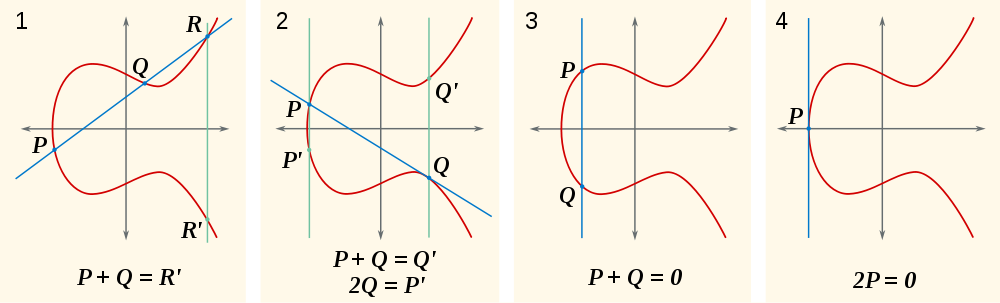
\includegraphics[width=\textwidth]{EllCurves}
\\
\\
The leftmost picture, labeled with $1$ shows that $P+Q=Q+P$, for it is easy to see that the line through $P$ and $Q$ remains the same.

The second picture ($2$) shows an expansion on the addition, wherein $Q+Q$ is calculated by taking the tangent to $Q$, arriving at $P$ which results in $Q+Q=P'$.

The third picture ($3$) shows both the existence of an inverse element, and the existence of a neutral element. Consider that any vertical line ends in the point $O$, the point at infinity. It is easy to see that the line through $O$ and $P$ ends up having a third point of intersection in $Q$, and that therefore $P+O=P$. Since it's already been shown that $P+O=P=O+P$ and therefore $O$ is the neutral element. Furthermore it is easy to see that $Q$ is the inverse element of $P$, since $P+Q=O$. Therefore it may be stated that $Q=-P$ and the existence of the inverse element has been proven.

The fourth picture ($4$) shows an interesting case, where the point on the curve at $x=0$ results in a point that is its own inverse, since $2P=O$ and $P-P=O$ so therefore in this case $P=-P$.
\\
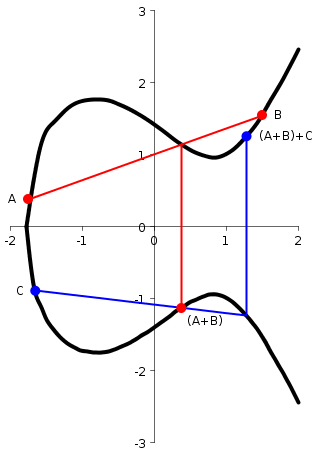
\includegraphics[width=0.5\textwidth]{EllAss1}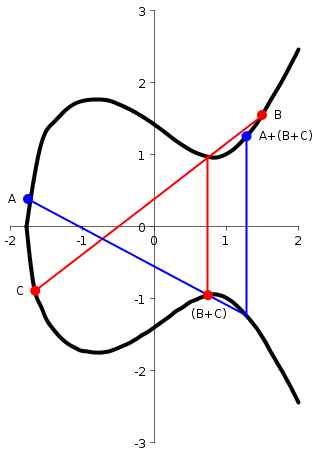
\includegraphics[width=0.5\textwidth]{EllAss2}
\\
\\
Finally associativity is shown by the two figures above. The left picture shows $(A+B)+C$, and the right picture shows $A+(B+C)$. It is easy to see that the points $A,B,C$ remained the same, and that, indeed, $(A+B)+C=A+(B+C)$.
\end{document}